\documentclass[oneside]{book}
\usepackage[utf8]{inputenc}
\usepackage{listings}
\usepackage{xcolor}
\usepackage{geometry}
\usepackage{mathtools}
\usepackage{listings}
\usepackage{hyperref}
\usepackage[ruled,vlined]{algorithm2e}
\usepackage{float}
\usepackage{import}
\geometry{margin=1in}

\begin{document}

\begin{titlepage}
	\centering 
	\scshape
	\vspace*{12\baselineskip}
	\rule{\textwidth}{1.6pt}\vspace*{-\baselineskip}\vspace*{2pt}
	\rule{\textwidth}{0.4pt} 
	\vspace{0.75\baselineskip}
	
	{\Large CS 406 : Algorithmic Graph Theory}{ \\\vspace{0.75\baselineskip} \LARGE Maximum Matching in Bipartite and General Graphs}
	\vspace{0.75\baselineskip}
	
	\rule{\textwidth}{0.4pt}\vspace*{-\baselineskip}\vspace{3.2pt} 
	\rule{\textwidth}{1.6pt}
	
	
	\vspace*{3\baselineskip}
	{\scshape\Large Bhargey Mehta\\ 201701074}
	
	\vspace{3\baselineskip} %originally 0.5
	
	
	\vspace{1\baselineskip} 
	
	\textit{\large Dhirubhai Ambani Institute of Information and Communication Technology \\ Gandhinagar\\} 
	


\end{titlepage}

\chapter{Introduction \& Motivation}
\section{Blossom Algorithm}
The blossom algorithm was developed by Jack Edmonds in 1965. It works on general unweighted graphs. The algorithm is named blossom because the odd length cycles are called blossoms.

The algorithm finds an application in the development of chemistry development kit. In organic chemistry a lot of focus is present on how bonds interact with each other since 2 compounds having the same molecular formula but different bond structure behave differently. While doing computational chemistry one often needs to assign the double bonds to specific places so that the valency of the carbon atoms is satisfied.

This can be posed as a problem in graph theory such that each carbon atom is a vertex and each single bond is an edge. Now we need to assign double bonds to certain singly bonded atoms. These double bonds cannot occur at a single vertex so a single vertex can belong to at maximum 1 double bond. This leads to the fact that the double bonds form a matching in the graph generated by a compound. This leads to a need to solve the maximum matching problem algorithmically in polynomial time.

\section{Hopcroft-Karp Algorithm}
The Hopcroft Karp Algorithm was developed by John Hopcroft and Richard Karp in 1973. It solves a specialised case of the assignment problem when the edge weights are equal i.e. we don't have a preference for any agent or job. This algorithm is of interest since it is faster than the Hungarian algorithm. Applications include matching organ donors to compatible patients, matching (same preference) job applicants to companies in a job fair etc.


\section{Hungarian Algorithm}
The Hungarian algorithm was developed by Harold Kuhn in 1955 and reviewed by James Munkres in 1957 to be polynomial time. Kuhn had developed this algorithm mainly on the basis of work done by Hungarian mathematicians Dénes Kőnig and Jenő Egerváry so he named the algorithm the "Hungarian" algorithm.

The algorithm works on a complete weighted bipartite graph. This is of interest because a well known combinatorial problem called the assignment problem can be posed as finding the maximum or minimum weighted matching in this bipartite setting. We are given a list of agents and a list of tasks. These lists of agents and tasks are nothing but the bipartitions of the graph. Each agent does the listed tasks for some cost which is the edge weight. We want to assign an agent to a single task so that the overall cost is maximum or minimum. This translates to finding a maximum weighted matching in the graph. Applications include assigning machines to factories, bidding and contract assignments etc.

\chapter{Blossom Algorithm}
% \documentclass{article}
% \usepackage[utf8]{inputenc}
% \usepackage{listings}
% \usepackage{xcolor}
% \usepackage{geometry}
% \usepackage{mathtools}
% \usepackage{listings}
% \usepackage{hyperref}
% \usepackage[ruled,vlined]{algorithm2e}
% \usepackage{float}
% \geometry{margin=1in}

% \begin{document}
\section{Algorithm}
Note that Blossom is a cycle of odd length and unsaturated vertex $v$ (wrt a matching $M$ of a graph $G$) is a node $v$ belongs to the graph $G$ but not present in matching $M$

\begin{algorithm}[!h]
\SetAlgoLined
\KwData{$G$, $M$}
\KwResult{$M^*$}
\caption{FindMaxMatching}

$P \leftarrow$ FindAugmentingPath($G$, $M$)

\If{$P$ is empty}{return $M$}

$M^+ \leftarrow$ increased matching of $M$ by adding alternating edges of $P$

return FindMaxMatching($G$, $M^+$)

\end{algorithm}


\begin{algorithm}[!h]
\caption{FindAugmentingPath}
\KwData{$G$, $M$}
\KwResult{$P$}

$F \leftarrow$ empty forest

rootOfNode $\leftarrow$ empty node-to-node mapping

terminals $\leftarrow$ unsaturated vertices of $G$

\For{each node $v$ in terminals}{
    Add $v$ to $F$
    
    rootOfNode($v$) $\leftarrow v$
}
    
mark all edges of $M$ in $G$

\For{each node $v$ in terminals}{
    \For{each unmarked edge $(v, w)$ adjacent to $v$}{
        \uIf{$w \notin F$}{
            AddToForest($M$, $F$, $v$, $w$, terminals, rootOfNode)
        }\uElse{
            $p_w \leftarrow$ rootOfNode($w$)
            
            \If{$d(w, p_w)$ is even}{
                $p_v \leftarrow$ rootOfNode($v$)
                
                \uIf{$p_v$ == $p_w$}{
                    $P \leftarrow$ BlossomRecursion($G, M, F, v, w$)
                }\uElse{
                    $P \leftarrow$ ConstructPath($F, v, w$, rootOfNode)   
                }
                return $P$
            }
        }
        
        mark edge $(v, w)$    
    }
}

return empty path
\end{algorithm}

\begin{algorithm}[!h]
\caption{Blossom Recursion}
\KwData{$G, M, F, v, w$}
\KwResult{$P$}

$B \leftarrow$ nodes in path from $v \to w$ in $F$

$G^+ \leftarrow G$ with all nodes of $B$ contracted into $w$

$M^+ \leftarrow M$ with all nodes of $B$ contracted into $w$

$P^+ \leftarrow$ findAugmentingPath($G^+, M^+$)

\If{$w \in P^+$}{
    $P \leftarrow$ liftBlossom($B, P^+, M$)

    return $P$
}

return $P^+$
\end{algorithm}

\begin{algorithm}[!h]
\caption{AddToForest}
\KwData{$M, F, v, w$, terminals, rootOfNode}
\KwResult{Null (Utility Function)}

$x \leftarrow$ node adjacent to $w$ in $M$

add edges $(v, w)$ and $(w, x)$ in $F$

add node $x$ in terminals

rootOfNode($w$) $\leftarrow$ rootOfNode($v$)

rootOfNode($x$) $\leftarrow$ rootOfNode($v$)
\end{algorithm}

\begin{algorithm}[H]
\caption{ConstructPath}
\KwData{$F, v, w$, rootOfNode}
\KwResult{$P$}

$p_v \leftarrow$ rootOfNode($v$)

$p_w \leftarrow$ rootOfNode($w$)

$P_1 \leftarrow$ Path from $v$ to $p_v$ in forest $F$

$P_2 \leftarrow$ Path from $v$ to $p_w$ in forest $F$

return $P_1 + P_2$
\end{algorithm}

\begin{algorithm}[!h]
\KwData{$B, P^+, M$}
\KwResult{$P$}
\caption{LiftBlossom}
$v \leftarrow$ node in $B$ such that it is incident on 2 edges not present in $M$

$x \leftarrow$ node in $B$ such that $(x, x') \in P^+$ but $(x, x') \notin M$

\If{no such $x$ exists}{return empty path}

$P_1 \leftarrow$ subpath of $P^+$ ending at $v$

$P_2 \leftarrow$ subpath of $P^+$ ending at $x$

$P_B \leftarrow$ path which begins at $(x, y)$ such that $(x, y) \in M$ and ends at $v$

$P \leftarrow P_1 + P_B + P_2$

return $P$
\end{algorithm}

\begin{figure}[!h]
    \centering
    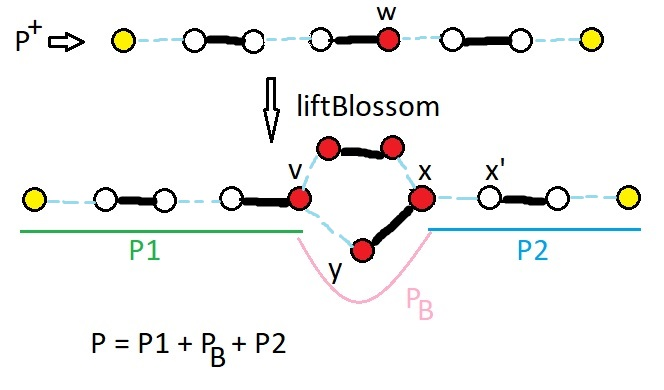
\includegraphics[scale=0.58]{lifting.jpg}
    \caption{Lifting a Blossom}
\end{figure}


\section{Proof of Correctness}
\subsection{Lemmas}
\subsubsection{Augmenting Path Lemma}
Given a graph $G$, a matching $M$ is maximum if and only if there is no augmenting path in $G$.

This lemma has been proved in lecture so we use it as it is.

\subsubsection{Identification Lemma}
Identification Lemma: This algorithm identifies Blossoms correctly.

The Blossom Recursion subroutine is executed only when the following conditions hold. This is because the conditions we impose before executing the said subroutine.
\begin{enumerate}
    \item Edge $(v, w)$ is unmarked.
    \item The parent of $v$ and $w$ is same i.e. $p_v = p_w$. Hence both are reachable from each other.
    \item Node $w$ is at an even distance from it's root $p_v$.
\end{enumerate}
Now there are 2 cases.
\begin{itemize}
    \item Case A: $v \in M$. 
        In this case $v$ must have been added to the list of terminal nodes by some other node and due to the structure of addToForest subroutine, we always add nodes which are at even distance from some original root of forest $F$. 
    \item Case B: $v \notin M$ or equivalently $v \in F$.
        In this case $v$ itself is a root and it's distance is 0, hence even.
\end{itemize}
Hence both $v$ and $w$ are at an even distance from $p_v$ and so the path that exists between them in $F$ is of even length. This path together with the edge $(v, w)$ forms a blossom.

\subsubsection{Base Lemma}
Since this blossom is formed of edges alternating in $M$ and length of the cycle is odd, there is exactly one node in blossom which is incident on 2 edges which are both absent in $M$ but present in the blossom. We call this vertex as the base of the blossom.

Stem Lemma: If the base is saturated by $M$, then the augmenting path $P^+$ which passes through the contracted blossom, passes through it such that it passes through the base.

The above lemma is true since, if it is not the case then it would imply that the vertex (which is not a base) is incident on 2 edges which are present in $M$ which contradicts the definition of $M$.

Note that in the figure above, node $v$ is the base of the blossom of size 5.

\subsection{Blossom Lemma}
Blossom Lemma: $G$ contains an augmenting path if and only if $G^+$ (the graph after contraction of blossom) contains an augmenting path.

Note that if the augmenting path in $G$ or $G^+$ doesn't pass through the blossom, then the proof is trivial since the path in both of them is exactly equal.

\subsubsection{Forward Proof}
There are 2 cases depending upon whether or not the blossom is internal to the augmenting path in $G^+$ or is an endpoint.
\begin{itemize}
    \item Case A: Blossom is internal to the augmenting path. 
        
        Observation $A_1$: Due to the base lemma proved above, there is one node which is the base (defined in lemma above) and hence the edge which enters into the blossom is in the matching.
        
        Observation $A_2$: Any other node is in the matching $M$ such that it's corresponding edge belongs to the matching and hence the edge which exits the blossom to the other end is not in the matching.
        
        From the above 2 observations, when the blossom is contracted into a single node, these 2 edges are alternating edges and hence the corresponding path in $G^+$ is augmenting.
    \item Case B: Blossom is an endpoint.
        
        Observation $A_2$ holds for this case also.
        
        Now since, the blossom is internal, the blossom becomes an unsaturated vertex since there is no edge incoming to this contracted blossom. 
        
        Hence we can say that the augmenting path in $G^+$ is aagain an augmenting path.
        
\end{itemize}


\subsubsection{Backward Proof}
Now since the blossom is of odd length, (WLOG) if we consider the base as the entry point and the other vertex as the exit point in the blossom, we can see that there are 2 paths (one travelling the upper path and the other travelling the lower path) between them. 

Independent of the position of the exit point wrt the entry point (base vertex), there is always a path of even length and a path of odd length. 

If we traverse from the base on the even length portion of the blossom, the first edge is not in the matching and the subsequent edges alternate. And since the path is of even length, the last edge is necessarily in matching.

Now again there are 2 cases.
\begin{itemize}
    \item Case A: Blossom is internal.
        
        According to the base lemma, the subpath outside the blossom attaching the unsaturated vertex to the base will end with an edge (incident on base) which is in the matching.
        
        For the edge connecting the exit point with the other unsaturated vertex, it is necessarily not in matching since the corresponding edge in matching $M$ belongs to the blossom.
        
        Hence in this case, the paths described above in union with the even length path forms an augmenting path in $G$.
    \item Case B: Blossom is and endpoint.
    
        For this case the first path in case A is an empty path and rest of the reasoning remains the same.
        
        Hence in this case also, the union of these paths forms an augmenting path in $G$.
\end{itemize}
Hence from the above Blossom Lemma in combination with the augmenting path lemma and the identification lemma, we can say that our algorithm is correct.

\section{Complexity Analysis}
\begin{itemize}
    \item The addToForest subroutine takes O(1) time since all 6 steps complete in constant time.
    \item The constructPath subroutine takes O($N$) time since the maximum length of a path can be $N$.
    \item The liftBlossom subroutine takes O($N$) time since the maximum length of the path can be $N$ and the decision to decide the subportion of the blossom to include in lifting the path is done in constant time.
    \item The findMaxMatching function is called recursively at max $\frac{N}{2}$ times since the size of the matching increases by 2 in every recursion call. Hence the time complexity is O$(N*$ cost of findAugmentingPath subroutine)
    \item Each call to the blossomRecursion subroutine will take at max O($N+M$) time barring the recursion since in each call the cost is equal to the size of the blossom found.
    \item In each call to the augmenting path finding algorithm, we either find a blossom and recurse or we find an augmenting path and return. We call the work done (traversing the edges and contraction of blossom) of O($N+M$) in the algorithm except the recursion work as a sub phase. Hence each recursion is a sub phase. There will be at most $O(N)$ sub phases. Hence the cost is O$(NM)$
\end{itemize}

Finally plug the above result in time complexity of findMaxMatching function. Hence overall time complexity of the entire algorithm is O$(N * O(M*N)) = $ O($N^2M$).

\section{Parallel Algorithm}
Now in the core subroutine given below, the outer for loop which iterates over vertices $v$ can't be parallelised since after each iteration, the state of the tree changes and hence there is an inherent dependency. However the inner loop which iterates over the adjacent edges of some vertex $v$ can be done in parallel. However in the sequential version, after processing one edge, we may either find a path (without the need of a Blossom Recursion) or we find no augmenting path and there is some blossom or there is no augmenting path. So if we allow each iteration to modify the forest in parallel, the state of the forest becomes inconsistent if one iteration finds a path and other doesn't. Hence we have to delay the actual modification of the forest until all edges have been processed. Note that this implies that we can't use the AddToForest subroutine.

\begin{algorithm}[!h]
\caption{FindAugmentingPath}
\KwData{$G$, $M$}
\KwResult{$P$}

$F \leftarrow$ empty forest

rootOfNode $\leftarrow$ empty node-to-node mapping

terminals $\leftarrow$ unsaturated vertices of $G$

\For{each node $v$ in terminals}{
    Add $v$ to $F$
    
    rootOfNode($v$) $\leftarrow v$
}

mark all edges of $M$ in $G$

\For{each node $v$ in terminals}{
    
    \textcolor{red}{temp $\leftarrow$ empty map}
    
    \For{each unmarked edge $(v, w)$ adjacent to $v$ \textcolor{red}{in PARALLEL}}{
        \uIf{$w \notin F$}{
            \textcolor{red}{$x \leftarrow$ node adjacent to $w$ in $M$}
        
            \textcolor{red}{temp($w$) $\leftarrow x$}
        }\uElse{
            $p_w \leftarrow$ rootOfNode($w$)
            
            \If{$d(w, p_w)$ is even}{
                $p_v \leftarrow$ rootOfNode($v$)
                
                \uIf{$p_v$ == $p_w$}{
                    $P \leftarrow$ BlossomRecursion($G, M, F, v, w$)
                }\uElse{
                    $P \leftarrow$ ConstructPath($F, v, w$, rootOfNode)   
                }
                return $P$
            }
        }
        
        mark edge $(v, w)$    
    }
    
    \For{\textcolor{red}{each node $w$ in temp in PARALLEL}}{
        \uIf{\textcolor{red}{$w ==$ temp(temp($w$))}}{
            \textcolor{red}{$P \leftarrow$ BlossomRecursion($G, M, F, v, w$)}
            
            \textcolor{red}{return $P$}
        }\uElse{
            \textcolor{red}{add edges $(v, w)$ and $(w, \mathrm{temp}(w)=x)$ in $F$}
            
            \textcolor{red}{add node $x=\mathrm{temp}(w)$ to terminals}
        }
    }
}

return empty path
\end{algorithm}

The maximum matching wrapper depends on the previous matching and so can't be parallelised however augmenting a matching can be done in parallel.

\begin{algorithm}[H]
\SetAlgoLined
\caption{FindMaxMatching}

$P \leftarrow$ FindAugmentingPath($G$, $M$)

\If{$P$ is empty}{return $M$}

$M^+ \leftarrow$ increased matching of $M$ by adding alternating edges of $P$ \textcolor{red}{in PARALLEL}

return FindMaxMatching($G$, $M^+$)
\end{algorithm}

The construct path algorithm is sequential by nature and hence can't be parallelised. The best we can do is find $P_1 \& P_2$ in parallel. This doesn't scale as the number of processors increases.

\begin{algorithm}[!h]
\caption{ConstructPath}
\KwData{$F, v, w$, rootOfNode}
\KwResult{$P$}

$p_v \leftarrow$ rootOfNode($v$)

$p_w \leftarrow$ rootOfNode($w$)

$P_1 \leftarrow$ Path from $v$ to $p_v$ in forest $F$ \textcolor{red}{in PARALLEL with $P_2$}

$P_2 \leftarrow$ Path from $v$ to $p_w$ in forest $F$ \textcolor{red}{in PARALLEL with $P_1$}

return $P_1 + P_2$
\end{algorithm}

In the below algorithm, the once the blossom is found, the contraction of the blossom can be done in parallel since the presence of each edge in the blossom is independent from other edges. The lifting algorithm remains unchanged due to dependencies in the path finding process.

\begin{algorithm}[!h]
\caption{Blossom Recursion}
\KwData{$G, M, F, v, w$}
\KwResult{$P$}

$B \leftarrow$ nodes in path from $v \to w$ in $F$

$G^+ \leftarrow G$ with all nodes of $B$ contracted into $w$ \textcolor{red}{in PARALLEL}

$M^+ \leftarrow M$ with all nodes of $B$ contracted into $w$ \textcolor{red}{in PARALLEL}

$P^+ \leftarrow$ findAugmentingPath($G^+, M^+$)

\If{$w \in P^+$}{
    $P \leftarrow$ liftBlossom($B, P^+, M$)

    return $P$
}

return $P^+$
\end{algorithm}

\subsection{Proof of Correctness}
we will consider the parallelism seen in the augmenting path finding algorithm since we're deviating from the serial counterpart.

When extending the forest in parallel, we are only considering the effect of adding one unmarked edge at a time. Since when processed in isolation, if blossoms are formed due to addition of this single edge then our algorithm is no different from the serial counterpart in terms of behaviour. Hence, to prove the correctness our algorithm, we only need to consider the case when a blossom is formed due to addition of edges from the same node $v$.

Suppose two edges $(v, w_i)$ and $(v, w_j)$ are some two edges. Their corresponding marked edges are $(w_i, x_i)$ and $(w_j, x_j)$. Note that $x_i$ and $x_j$ are BOTH not present in the forest at this moment since if one of them were present then we would found a blossom while considering the other, before reaching at this situation. Both $(v, w_i)$ and $(v, w_j)$ are unmarked so $v$ is necessarily the base of the blossom. Now consider the following 2 cases:
\begin{itemize}
    \item Blossom is of size 5 or greater: If it is blossom of size 5 or more then the remaining part of the blossom should already be present in the forest since we have just added 3 edges and discovered a blossom. But this leads to a contradiction to our original assumption that $x_i$ and $x_j$ were both absent in the forest.
    \item Blossom is of size 3: From above, we can see that the blossom formed would always be a size 3 blossom. We are specifically checking for size 3 blossom in our algorithm after the edges are handled in parallel.
\end{itemize}

\subsection{Time Complexity}
\begin{itemize}
    \item There will be at max O($|V|$) iterations of the main algorithm since a matching of size at max $\frac{|V|}{2}$ is possible.
    \item We now again examine the work done in each sub phase of the algorithm. We have to iterate over all the vertices and then their edges in parallel. This means work of O($|V|\frac{|V|}{p}$).
    \item In the same sub phase, the work done by the blossom recursion is O($|V|+\frac{|E|}{p}$) since the blossom identification cannot be parallelised.
    \item Each sub phase thus takes O($|V|+|V|\frac{|V|}{p} + \frac{|E|}{p}$) task. There can be at most O($V$) of these sub phases. Hence total time of the augmenting path finding algorithm takes O($|V|^2 + \frac{|V|^3}{p} + \frac{|V||E|}{p}$)
\end{itemize}
Hence the overall time complexity would be O($|V| \times (|V|^2 + \frac{|V|^3}{p} + \frac{|V||E|}{p})$) = O$(|V|^3 + \frac{|V|^4}{p} + \frac{|V|^2|E|}{|p|^2})$.

\section{Distributed Algorithm}
As discussed earlier, due to the sequential nature of the algorithm, it is very difficult to parallelise the blossom algorithm. In the blossom contraction, several edges have to be collapsed into a single node. This requires that the graph be modified and further recursions be applied upon this modified graph. 

In a distributed setting this requires some central authority that handles this contraction. We will be using 2 algorithms $A_1$ and $A_2$. $A_1$ rebuilds the graph locally be obtaining the information from the network and then applies $A_2$ locally to produce the required result. 

The algorithm $A_2$ would be the blossom algorithm in our case. We are assuming that a single vertex can contain the information of the entire network and there is a authority vertex which drives the collection of the network information and then runs the blossom algorithm locally.

\begin{algorithm}[!h]
\caption{$A_1$: Build network}
\KwData{authority vertex id $v_a$ and own id $v$}

$C \leftarrow $ empty set

\uIf{$v == v_a$}{
    $p \leftarrow $ NULL
    
    \For{each adjacent $w$}{
        send DISCOVER msg
    }
    \For{each adjacent $w$}{
        receive DISCOVERY\_RESULT
        
        \If{DISCOVERY\_RESULT is accepted}{
            add $w$ to $C$    
        }
    }
    \For{each adjacent $w$}{
        receive DISCOVER msg
        
        send DISCOVERY\_REJECTED to $w$
    }
    \For{each $c_i \in C$}{
        receive ADJACENCY\_INFO from $c_i$
    }
    run the BLOSSOM ALGORITHM locally
    
    print the result and shut down
}\uElse{
    receive 1 DISCOVER msg from some $w$
    
    send DISCOVERY\_ACCEPTED to $w$
    
    $p \leftarrow w$
    
    \For{each adjacent $w$ except $p$}{
        send DISCOVER msg
    }
    \For{each adjacent $w$ except $p$}{
        receive DISCOVERY\_RESULT
        
        \If{DISCOVERY\_RESULT is accepted}{
            add $w$ to $C$
        }
    }
    \For{each adjacent $w$ except $p$}{
        receive DISCOVER msg
        
        send DISCOVERY\_REJECTED to $w$
    }
    
    subTreeInfo $\leftarrow$ NULL
    
    \For{each $c_i \in C$}{
        receive ADJACENCY\_INFO from $c_i$
        
        subTreeInfo $\leftarrow$ subTreeInfo $\cup$ ADJACENCY\_INFO 
    }
    
    send subTreeInfo to $p$ and shut down
}
\end{algorithm}

\subsection{Correctness and Message Complexity}
The algorithm works by sending a discovery message to all adjacent neighbours. Neighbours which have not been discovered would then reply their parents with an accepted response. This way a parent-child relationship is established which forms a DFS tree in the network. 

Now the vertex itself sends discovery message to its neighbours to determine its children and so on. Any new discovery message is responded with a discovery reject response.

In this DFS network, the leaf nodes will first send their adjacency info to their parents since their child set $C$ would be empty. The vertices which are internal will wait for all children to send them adjacency information. This would contain the the network information of all the children, grand-children etc of that vertex. This vertex now unions this information with its own adjacency list and then forwards it to their parent. In this way the entire network is now accumulated at the driver node $v_a$ which then runs the blossom algorithm locally.

Along each edge we have 3 messages- discovery, discovery result and adjacency information hence the message complexity of the algorithm would be O($3|E|$).



\section{References}
\begin{itemize}
    \item \href{https://stanford.edu/~rezab/classes/cme323/S16/projects_reports/shoemaker_vare.pdf}{\color{blue} Blossom Algorithm Analysis by Amy Shoemaker \& Sagar Vare}
    \item \href{https://en.wikipedia.org/wiki/Blossom_algorithm}{\color{blue} Wikipedia Blossom Algorithm}
\end{itemize}



%\end{document}


\chapter{Hopcroft-Karp Algorithm}
\newpage
\documentclass{article}
\usepackage[utf8]{inputenc}
\usepackage{listings}
\usepackage{xcolor}
\usepackage{geometry}
\usepackage{mathtools}
\usepackage{listings}
\usepackage{hyperref}
\usepackage[ruled,vlined]{algorithm2e}
\usepackage{float}
\geometry{margin=1in}

\begin{document}

\section{Algorithm}
We will be using the Hopcroft-Karp algorithm which produces a maximum matching in a bipartite graph. Note that $X$ and $Y$ are the bipartitions of the bipartite graph $G$ and $M$ is some matching of $G$. If $G$ has a perfect matching then any maximum matching is also a perfect matching.

\vspace{0.5cm}

\begin{algorithm}[!h]
\caption{BFS}
\KwData{$X, Y, M$}
\KwResult{$G_{\mathrm{BFS}}$}

$G_{\mathrm{BFS}} \leftarrow$ empty graph

visited $\leftarrow$ empty Set

$Q \leftarrow$ empty Queue

\For{each node $v$ in $B_1$}{
    \If{$v \notin M$}{
        enqueue $v$ in $Q$

        add $v$ to visited
    }
}
\While{$Q$ is NOT empty}{

    $v \leftarrow$ dequeue from $Q$

    \uIf{$v \in X$}{
        \For{each edge $(v, w)$ adjacent to $v$ such that $(v, w) \notin M$}{
            add $(v, w)$ to $G_{\mathrm{BFS}}$
        
            enqueue $w$ in $Q$
        
            add $w$ to visited   
        }
    }\uElse{
        \For{each edge $(v, w)$ adjacent to $v$ such that $(v, w) \in M$}{
            add $(v, w)$ to $G_{\mathrm{BFS}}$
    
            enqueue $w$ in $Q$
    
            add $w$ to visited       
        }
    }
}

return $G_{\mathrm{BFS}}$
\end{algorithm}

\begin{algorithm}[!h]
\KwData{$G_{\mathrm{BFS}}, M, v$, visited, $P$}
\KwResult{Boolean}
\caption{ActualDFS}
\If{$v$ in visited}{return False}

add $v$ to visited

\For{all edges $(v, w)$ adjacent to $v$ in $G_{\mathrm{BFS}}$}{
    \If{($v \in X$ and $(v,w) \notin M$) or ($v \in Y$ and $(v,w) \in M$)}{skip edge}
    
    append $(v, w)$ to $P$
    
    \If{$w \notin M$}{
        add $w$ to visited
        return True
    }
    
    foundPath $\leftarrow$ actualDFS($G_{\mathrm{BFS}}, M, w$, visited, $P$)
    
    \If{foundPath is True}{return True}
    
    remove $(v, w)$ from $P$
}
return False
\end{algorithm}

\begin{algorithm}[!h]
\caption{DFS (wrapper)}
\KwData{$G_{\mathrm{BFS}}, M$}
\KwResult{set of disjoint paths}

visited $\leftarrow$ empty set

disjointPaths $\leftarrow$ empty set

\For{each node $v$ in $Y$}{
    \If{$v \notin M$}{
        $P \leftarrow$ empty path 

        ActualDFS($G_{\mathrm{BFS}}, M, v$, visited, $P$)

        add $P$ to disjointPaths if $P$ is NOT empty
    }
}
return disjointPaths
\end{algorithm}

\begin{algorithm}[!h]
\SetKwRepeat{Do}{do}{while}
\caption{HopcroftKarp}
\KwData{$X, Y, G$}
\KwResult{$M^*$}

$M \leftarrow$ empty matching

\Do{disjointPaths is NOT empty}{
    $G_{\mathrm{BFS}} \leftarrow$ BFS($X, Y, M$)

    disjointPaths $\leftarrow$ DFS($G_{\mathrm{BFS}}, M$)
    
    augment $M$ with each $P$ in disjointPaths
}
return $M$
\end{algorithm}


\section{Proof of Correctness}
\subsection{Augmenting Path Lemma}
Augmenting Path Lemma: A matching $M$ of $G$ is maximum if and only if there is no augmenting path in $G$.

This lemma has been proved in the lecture, so we use it as it is.

\subsection{Disjoint Paths Lemma}
Disjoint Path Lemma: The paths returned by the DFS subroutine are vertex disjoint and are augmenting paths of $M$ wrt $G$.

\begin{figure}[!h]
    \centering
    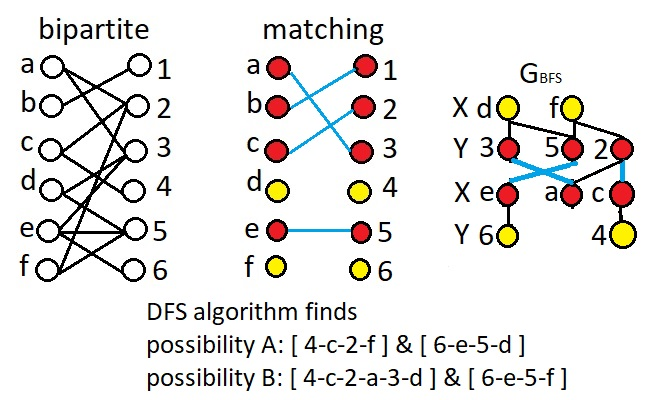
\includegraphics[scale=0.7]{hopcroftkarp_bfs.jpg}
    \caption{Finding Augmenting Paths}
\end{figure}

The graph formed by the BFS has 2 types of nodes, belonging to $X$ and belonging to $Y$. They can be imagined as stacks of layers going from top to bottom as shown in the figure. It is easy to see that the algorithm selects edges going from $X \to Y$ only when the edge is NOT present in the matching and selects edges going from $Y \to X$ only when the edge IS present in the matching.

Hence when we apply DFS from a node $v \in Y$, we are guaranteed to find a node $w \in X$ and $w \in M$ such that $(v, w) \notin M$. Similarly when we move from a node $v \in X $ and $v \in M$, we are guaranteed to find a node $w \in Y$ such that $(v, w) \in M$.

Also see that the DFS returns a path which begins and ends at nodes NOT present in the matching. Further the path contains edges alternate between $X$ and $Y$ such that all edges from $X \to Y \in M$ and all edges from $Y \to X \notin M$. Hence this path is an augmenting path.

Moreover this path is also disjoint since after using a node we immediately mark it as used. Hence it is effectively removed from the graph $G_{\mathrm{BFS}}$ and cannot be shared with any other path found by further iterations of the DFS algorithm.

\section{Time Complexity}

\subsection{Claim 1}
We make a claim that for a maximum matching $M^*$ and some matching matching $M$, the symmetric difference of $M^*$ and $M = M \Delta M^*$ has $|M^*|-|M|$ augmenting paths and these paths are vertex disjoint. 

We know that the presence of an augmenting path increases the size of $M$ by 1. So there are exactly $|M^*|-|M|$ augmenting paths. Also since the degree of each node is at max 2, the paths are vertex-disjoint.

\subsection{Claim 2}
We make a claim that there are at max $2\sqrt{N}$ iterations in the main loop. 

Notice that each iteration of the main algorithm increases the size of the matching by at least 1. Hence the shortest augmenting path is of length $\sqrt{N}$ after $\sqrt{N}$ iterations.

Since these paths will be vertex disjoint, we can say that there are at maximum $\sqrt{N}$ augmenting paths. Each of these paths increases the size of $M$ by 1 and hence $|M^*|-|M|$ is at max $\sqrt{N}$. Hence optimal matching $M^*$ will be achieved after at max $\sqrt{N}$ more iterations of the main algorithm.

\subsection{Calculating Time Complexity}
\begin{itemize}
    \item Each iteration involves BFS, DFS and augmenting $M$ with vertex disjoint paths.
    \item Both BFS and DFS take O$(|E|)$ time.
    \item Since the paths used to augment $M$ are vertex disjoint, the entire process takes O$(|V|)$ time.
    \item Hence each iteration of the main algorithm takes O$(|V|+|E|)$ = O($|E|$) time.
    \item From claim 2, we can see that there are at max O$(\sqrt{|V|})$ iterations.
\end{itemize}
So the overall time complexity is O($|E|\sqrt{|V|}$).

\section{Parallel Hopcroft-Karp Algorithm}
The main 2 components of the Hopcroft-Karp Algorithm are augmenting the matching and disjoint path finding in the bipartite graph. The augmentation of the matching is has a dependency i.e. to augment some matching, we need the matching itself. 

The second component i.e. disjoint path finding again consists of a modified BFS and DFS. Attempting the BFS in a prallel manner results in the need of synchronisation between the processors at such a high level that the parallelism is negligible even when ignoring overheads. Similarly is the case for DFS. To make the paths vertex disjoint we have to make use of mutual exclusion when considering the neighbours of a vertex. This again results in overheads (checking all neighbours of a vertex before performing the recursion) in the algorithm that actually increase the time complexity. 

However experiments have shown that using these techniques, an experimental speedup is obtained even with a poorer time complexity than the serial algorithm.

\section{References}
\href{https://en.wikipedia.org/wiki/Hopcroft\%E2\%80\%93Karp_algorithm}{\textcolor{blue}{Hopcroft-Karp Algorithm Wikipedia (Clickable URL)}}

\href{https://people.eecs.berkeley.edu/~aydin/matchingGraft.pdf}{\textcolor{blue}{A Parallel Tree Grafting Algorithm for Maximum Cardinality Matching in Bipartite Graphs by Ariful Azad, Aydin Buluc, Alex Pothen}}




\end{document}


\chapter{Hungarian Algorithm}
\newpage
\documentclass{article}
\usepackage[utf8]{inputenc}
\usepackage{listings}
\usepackage{xcolor}
\usepackage{geometry}
\usepackage{mathtools}
\usepackage{listings}
\usepackage{hyperref}
\usepackage[ruled,vlined]{algorithm2e}
\usepackage{float}
\geometry{margin=1in}

\begin{document}
\section{Introduction}
We are given a complete bipartite graph $G$ with $|X|=|Y|$ such that $X$ denotes the jobs and $Y$ denotes the agents. The edge weight $w(x, y)$ of edge $e(x, y)$ denotes the cost of doing job $y$ when assigned to agent $x$.

We will first clarify some terminologies related to the algorithm.

\subsection{Alternating Tree}
A sub graph of $G$ which is a tree having an unsaturated root wrt some matching $M$ having the edges alternate between being in $M$ and not being in $M$ is called an alternating tree. Hence we can see that if a leaf node is unsaturated in this alternating tree, then the path from root to this leaf node is an augmenting path.

\subsection{Labelling Function}
A labelling function is a mapping $l: V \to Z$ such that it assigns an integer to each node in $G$. Hence $l(v)$ denotes the label of node $v \in G$.

A labelling is called feasible if for every edge $e(x, y)$ we have,
$$l(x)+l(y) \geq w(x, y)$$.

\subsection{Equality Graph}
Let $E_l$ denote the set of edges $e(x, y)$ such that wrt some labelling function $l$, the equality $l(x)+l(y) = w(x, y)$ holds.

The graph $G_l$ formed by the vertices of $G$ and the edge set $E_l$ is called the equality graph $G_l$ wrt the labelling function.

\section{Lemmas}

\subsection{Kuhn-Munkres Lemma}
The Kuhn-Munkres Lemma (abbreviated as KM Lemma from now on) is at the heart of this algorithm. It states that,

KM Lemma: If $l$ is a feasible labelling and $M$ is a perfect matching in $G_l$ then $M$ is maximum weight matching in $G$.

Let $M'$ be any perfect matching in $G$ not necessarily maximum and not necessarily in $G_l$. We have the weight $w(M') = \Sigma w(x, y)$ where $e(x, y) \in M'$.

Since $M'$ is a perfect matching, each vertex appears only once in this summation. Since $l$ is feasible, we have $w(x, y) \leq l(x)+l(y)$, we get the following result.

$$w(M') = \Sigma w(x, y) \leq \Sigma l(v)$$.

Now consider a perfect matching $M$ in $G_l$. Note that by definition of $G_l$ we have $w(x, y) = l(x)+l(y)$. Hence we get the following result.

$$w(M) = \Sigma w(x, y) = \Sigma l(v)$$

Combining these results we get $W(M) \geq W(M')$ and hence $M$ is maximum weight matching in $G$.

\subsection{Relabelling Lemma}
We will now look at a relabelling lemma which will aid is in modifying a given feasible $l$ into another feasible labelling $l'$.

If $S \subseteq X$ then let $N_l(S)$ denote the set of vertices $v \in Y$ such that for some $u \in X$, $e(u, v) \in E_l$.

Relabelling Lemma: Let $S \subseteq X$ and let $T=N_l(S) \neq Y$, we have $$\alpha_l = \mathrm{min}(\{l(x)+l(y)-w(x, y) : x \in S, y \notin T\})$$

$$l'(v) = 
\begin{cases}
l(v)-\alpha_l & v \in S \\
l(v)+\alpha_l & v \in T \\
l(v) & \mathrm{otherwise} \\
\end{cases} $$ 

is a feasible labelling such that
\begin{enumerate}
    \item If $e(x, y) \in L$ such that $x \in S, y \in T$, then $e(x, y) \in E_{l'}$.
    \item If $e(x, y) \in L$ such that $x \notin S, y \notin T$, then $e(x, y) \in E_{l'}$.
    \item $\exists$ edge $e(x, y)$ with $x \in S, y \notin T$ such that $e(x, y) \in E_{l'}$ 
\end{enumerate}

Proof
\begin{enumerate}
    \item $x \in S, y \in T$: The same amount is added on one side and subtracted on another so the sum remains the same. If $e(x, y) \in E_l$, then $l(x)+l(y) = w(x, y) = (l(x)-\alpha_l)+(l(y)+\alpha_l)$.
    \item $x \in S, y \notin T$: In this case, for each edge, we have some slack about how much we can reduce $l(x)$, since $\alpha_l$ is the minimum of that slack, the labelling remains feasible. In addition the edge\/s which correspond to the minimum slack are now present in $E_{l'}$.
    \item $x \notin S, y \in T$: In this case the label of $y$ is being increased by $\alpha_l$ hence $l'$ remains feasible.
    \item $x \notin S, y \notin T$: The labelling remains the same, hence it is feasible.
\end{enumerate}

\section{Algorithm}

\begin{algorithm}[!h]
\KwData{$G$}
\KwResult{$M^*$}
\caption{HungarianMatching}

$M \leftarrow$ empty matching

\For{all $x \in X$}{$l(x)\leftarrow$ max($w(x, y)$)}

\For{all $y \in Y$}{$l(y) \leftarrow 0$} 

\While{$M$ is not perfect matching}{
    $P, l \leftarrow$ FindAugmentingPath($G$, $l$, $M$)

    $M \leftarrow$ augment $M$ with $P$
}
return $M$
\end{algorithm}

\begin{algorithm}[!h]
\caption{FindAugmentingPath}
\KwData{$G$, $l$, $M$}
\KwResult{$P, l^*$}

pick unsaturated vertex $u \in X$

$S \leftarrow \{u\}$ and $T \leftarrow \phi$

$P \leftarrow$ NULL

\While{$P$ is NULL (path not found)}{
    \If{$N_l(S) = T$}{
        $\alpha_l \leftarrow \mathrm{min}(\{l(x)+l(y)-w(x, y) : x \in S, y \notin T\})$

        $l^*(v) \leftarrow 
        \begin{cases}
        l(v)-\alpha_l & v \in S \\
        l(v)+\alpha_l & v \in T \\
        l(v) & \mathrm{otherwise} \\
        \end{cases}$
    }
    $l \leftarrow l^*$

    pick one $v$ from $\in N_l(S)-T$
    
    \uIf{$v$ is unsaturated}{$P \leftarrow$ path from $v$ to root $u$}
    \uElse{
    
        $z \leftarrow$ the matched vertex of $v$ by edge $e(v, z) \in M$

        $S \leftarrow S \cup \{z\}$ and $T \leftarrow T \cup \{v\}$
    }
}
return $P, l^*$
\end{algorithm}

\section{Proof of Correctness}
It is easy to see that the initial labelling function is feasible. 

We claim that the alternating tree $T_u$ rooted $u$ in the augmenting path finding algorithm is always contained in the labelling even after we modify the labelling according to the relabelling lemma. This claim can be proved by induction as below.
\begin{itemize}
    \item Base Case: $T_u$ only contains $u$. It is trivial to see that the claim holds.
    \item Assume that the edges of $T_u$ are in $E_l$. Note that this is equivalent to saying $T_u \cap X = S$ and $T_u \cap Y = T$. But this means that every edge in $T_u$ is such that one of its end points is in $S$ and another in $T$. Hence by reason \#1 of the relabelling lemma explained in section 2, all these edges are present in $E_{l^*}$ as well.
    \item We also add new edges but those are already according to the updated labelling and hence present $T_u$ according to $E_{l^*}$ as well.
\end{itemize}

Hence we prove that our alternating tree $T_u$ always increases in size. And since $M$ was not perfect, we are guaranteed to find an unsaturated vertex $z$ eventually which would provide us the augmenting path $P$..

Note that we are always selecting edges from the set $E_l$ and by definition these edges are present in $G_l$. We have also proved in the relabelling lemma that the modified labelling is always feasible and have also proved by induction that the edges are always present in the modified labelling. 

This means that the matching eventually becomes a perfect matching in $G_l$ and by the KM Lemma proved earlier in section 2, the resultant matching will be a maximum weight matching in $G$.

\section{Time Complexity}
\begin{enumerate}
    \item In the augmenting path finding algorithm, the augmenting path would be found after at max O$(|V|)$ iterations of the outer loop.
    \item The minimum of the slacks i.e. $\alpha_l$ can be found in O($|V|$) time and all the new labelling can be obtained after O($|V|$) updates. Adding $v$ to $T$ and $z$ to $S$ is constant time task Hence one single iteration takes O($|V|$) time.
    \item The overall time complexity of the path finding algorithm is O($|V|^2$) since there are O($|V|$) iterations each costing O($|V|$) time.
    \item The Hungarian algorithm augments the matching. A single augmentation increases the size of the matching by 1 and hence there will be O($|V|$) iterations of the path finding algorithm.
\end{enumerate}
Thus the overall time complexity of the Hungarian algorithm would be O($|V|^3$).

\section{Parallel Hungarian Algorithm}
Like in the above algorithms, Hungarian algorithm's path augmenting step cannot be parallelised due to the matching dependency. When considering the augmenting path algorithm, it contains finding minimum and updates of slacks.

The updates of slacks can be done in parallel. Finding the minimum of the slacks in parallel can take O($\frac{|V|}{p}+p$). Thus the time complexity could then be reduced to O($|V|^2(\frac{|V|}{p}+p)$) = O($p|V|^2 + \frac{|V|^3}{p}$).

\section{References}

\begin{itemize}
    \item \href{http://www.cse.ust.hk/~golin/COMP572/Notes/Matching.pdf}{\textcolor{blue}{Notes by Dr. Mordecai J Golin (Clickable URL)}}
\end{itemize}


\end{document}

\chapter{Related Algorithms}
\section{Unweighted Maximum Matching in Bipartite Graphs}
\begin{itemize}
    \item \href{https://epubs.siam.org/doi/10.1137/0202019}{\textcolor{blue}{1973: J Hopcroft, R Karp; An $N^{\frac{5}{2}}$ Algorithm for Maximum Matchings in Bipartite Graphs}}
    \item \href{https://www.sciencedirect.com/science/article/abs/pii/002001909190195N}{\textcolor{blue}{1991: H Alt, N Blum, K Mehlhorn, M Paul; Computing a maximum cardinality matching in a bipartite graph in time O($n^{1.5}m\log n$)}}
    \item \href{https://www.sciencedirect.com/science/article/pii/S0022000085710653}{\textcolor{blue}{1995: T Feder, R Motwani; Clique Partitions, Graph Compression and Speeding-Up Algorithms}}
\end{itemize}

\section{Weighted Maximum Matching in Bipartite Graphs}
\begin{itemize}
    \item \href{https://onlinelibrary.wiley.com/doi/abs/10.1002/nav.3800020109}{\textcolor{blue}{1955: H Kuhn ; The Hungarian method for the assignment problem}}
    \item \href{https://www.orsj.or.jp/~archive/pdf/e_mag/Vol.03_01_02_027.pdf}{\textcolor{blue}{1960: M Iri; A New Method for Solving Transportation-Network Problems}}
    \item \textcolor{blue}{1969: E Dinic, M Konrod; An Algorithm for the Solution of the Assignment Problem}
    \item \href{https://www.sciencedirect.com/science/article/pii/002200008590039X}{\textcolor{blue}{1985: H Gabow; Scaling algorithms for network problems}}
    \item \href{https://dl.acm.org/doi/10.1145/28869.28874}{\textcolor{blue}{1987: M Fredman, R Tarjan; Fibonacci heaps and their uses in improved network optimization algorithms}}
    \item \href{https://epubs.siam.org/doi/10.1137/0218069}{\textcolor{blue}{1989: H Gabow, R Tarjan; Faster Scaling Algorithms for Network Problems}}
    \item \href{https://link.springer.com/chapter/10.1007\%2F3-540-48481-7_38}{\textcolor{blue}{1999: M Kao, T Lam, W Sung, H Ting; A Decomposition Theorem for MaximumWeight Bipartite Matchings with Applications to Evolutionary Trees}}
    \item \href{https://epubs.siam.org/doi/10.1137/S0097539799361208}{\textcolor{blue}{2001: M Kao, T Lam, W Sung, H Ting; A Decomposition Theorem for Maximum Weight Bipartite Matchings}}
    \item \href{https://link.springer.com/chapter/10.1007\%2F978-3-319-06089-7_22}{\textcolor{blue}{2014: S Das, K Kapoor; Fine-Tuning Decomposition Theorem for Maximum Weight Bipartite Matching}}
\end{itemize}

\newpage
\section{Unweighted Maximum Matching in General Graphs}
\begin{itemize}
    \item \href{https://link.springer.com/chapter/10.1007/978-0-8176-4842-8_26}{\textcolor{blue}{1965: J Edmonds; Paths, Trees and Flowers}}
    \item \href{https://dl.acm.org/doi/10.1145/321941.321942}{\textcolor{blue}{1972: H Gabow; An Efficient Implementation of Edmonds' Algorithm for Maximum Matching on Graphs}}
    \item \href{https://link.springer.com/article/10.1007/BF02239502}{\textcolor{blue}{1974: T Kameda, I Munro; A O($|V||E|$) algorithm for maximum matching of graphs}}
    \item \href{https://dl.acm.org/doi/10.1109/SFCS.1975.5}{\textcolor{blue}{1975: S Even, O Kariv; An O($N^{2.5}$) algorithm for maximum matching in general graphs}}
    \item \href{https://dl.acm.org/doi/10.1109/SFCS.1980.12}{\textcolor{blue}{1980: S Micali, V Vazirani; An O($\sqrt{|V|}|E|$) algoithm for finding maximum matching in general graphs}}
\end{itemize}

\section{Completely Distributed Algorithms}
It is interesting to note that completely distributed maximum matching algorithms which have no sequential counterpart were not found. One of the reason could be that all these algorithms make use of the fact that a matching would have an augmenting path in case it is not maximum which is a property of the graph that turns up at a global level.

\chapter*{References}
All the references used to create this report are listed below. The references are hyperlinks.
\begin{enumerate}
    \item \href{https://people.eecs.berkeley.edu/~aydin/matchingGraft.pdf}{\textcolor{blue}{Ariful Azad, Aydin Buluc, Alex Pothen (2015); A Parallel Tree Grafting Algorithm for Maximum Cardinality Matching in Bipartite Graphs}}
    \item \href{https://link.springer.com/article/10.1007\%2FBF01840395}{\textcolor{blue}{Michael M. Wu; Michael C. Loui (1990). An efficient distributed algorithm for maximum matching in general graphs}}
    \item \href{https://en.wikipedia.org/wiki/Hopcroft\%E2\%80\%93Karp_algorithm}{\textcolor{blue}{Wikipedia Article on the Hopcroft-Karp Algorithm}}
    \item \href{https://en.wikipedia.org/wiki/Blossom_algorithm}{\color{blue} Wikipedia Article on the Blossom Algorithm}
    \item \href{https://stanford.edu/~rezab/classes/cme323/S16/projects_reports/shoemaker_vare.pdf}{\color{blue} Amy Shoemaker \& Sagar Vare (2016); Edmond's Blossom Algorithm}
    \item \href{http://www.cse.ust.hk/~golin/COMP572/Notes/Matching.pdf}{\textcolor{blue}{Dr. Mordecai J Golin; Notes on the Hungarian Algorithm}}
    \item \href{https://en.wikipedia.org/wiki/Hungarian_algorithm}{\textcolor{blue}{Wikipedia Article on the Hungarian Algorithm}}
    \item \href{https://baoilleach.blogspot.com/2017/08/my-acs-talk-on-kekulization-and.html}{\textcolor{blue}{Noel O'Boyle, John Mayfield (2017); ACS Talk}}
    \item \href{https://arxiv.org/pdf/1411.1919.pdf}{\textcolor{blue}{R Duan, S Pettie, H Su (2014); Scaling Algorithms for Weighted Matching in General Graphs}}
    \item \href{https://www.researchgate.net/publication/343998266_A_Modified_Decomposition_Algorithm_for_Maximum_Weight_Bipartite_Matching_and_Its_Experimental_Evaluation}{\textcolor{blue}{S Das (2020); A Modified Decomposition Algorithm for Maximum Weight Bipartite Matching and Its Experimental Evaluation}}
\end{enumerate}

\end{document}